\documentclass[3p]{elsarticle}
\usepackage{ae,aecompl}
\usepackage[T1]{fontenc}
\usepackage[utf8]{inputenc}
\usepackage{pgfplots}
\usepackage{pst-plot}
\usepackage{tikz}
\usepgfplotslibrary{external}
\tikzexternalize
\usepackage{amsmath}
\usepackage{amssymb}
\usepackage{gensymb}
\usepackage{upgreek}
\usepackage{float}
\usepackage{indentfirst}
\parskip=0pt

\begin{document}

\begin{frontmatter}

\title{The effect of electric field on potentiometric Scanning Electrochemical Microscopic images}
\cortext[cor]{Corresponding author}
\author[akiss]{András Kiss\corref{cor}}
\address[akiss, gnagy]{Department of General and Physical Chemistry, Faculty of Sciences, University of Pécs, 7624 Pécs, Ifjúság útja 6, Hungary}
%\address[akiss, gnagy]{János Szentágothai Research Centre, University of Pécs, 7624 Pécs, Ifjúság Útja 20, Hungary}
\ead{akiss@gamma.ttk.pte.hu}
\author[dfilotas]{Dániel Filotás}
\ead{filotasdaniel@gmail.com}
\author[gnagy]{Géza Nagy}
\ead{g-nagy@gamma.ttk.pte.hu}


\begin{abstract}

Scanning Electrochemical Microscopy (SECM) is an invaluable tool in corrosion science.
It allows the selective imaging of a particular ionic species being released at the anodic sites, using ion-selective microelectrodes (ISMEs) as scanning probes.
An often studied phenomenon is galvanic corrosion, which involves two metals in electrical contact, immersed in the same electrolyte.
The measured potential of the ISME is thought to depend only on the activity of primary ion.
However, an electric field is also formed as a result of the potential difference between the surfaces of the galvanic pair, which has a direct influence on the potential of the microelectrode.
Therefore, the measured potential is the sum of these two.
The potential difference caused by the electric field can be substantially large, exceeding that of the potential difference associated with the activity of the primary ion.
In this paper, we present experimental evidence of this, and investigate the extent to which it influences the final image. 
\end{abstract}
\begin{keyword}
	scanning electrochemical microscopy \sep potentiometry \sep galvanic corrosion \sep electric field
\end{keyword}
\end{frontmatter}

\section{Introduction}
Citation \cite{artefacts}.

\begin{figure}[h!]
\centering
% trim = top left bottom right
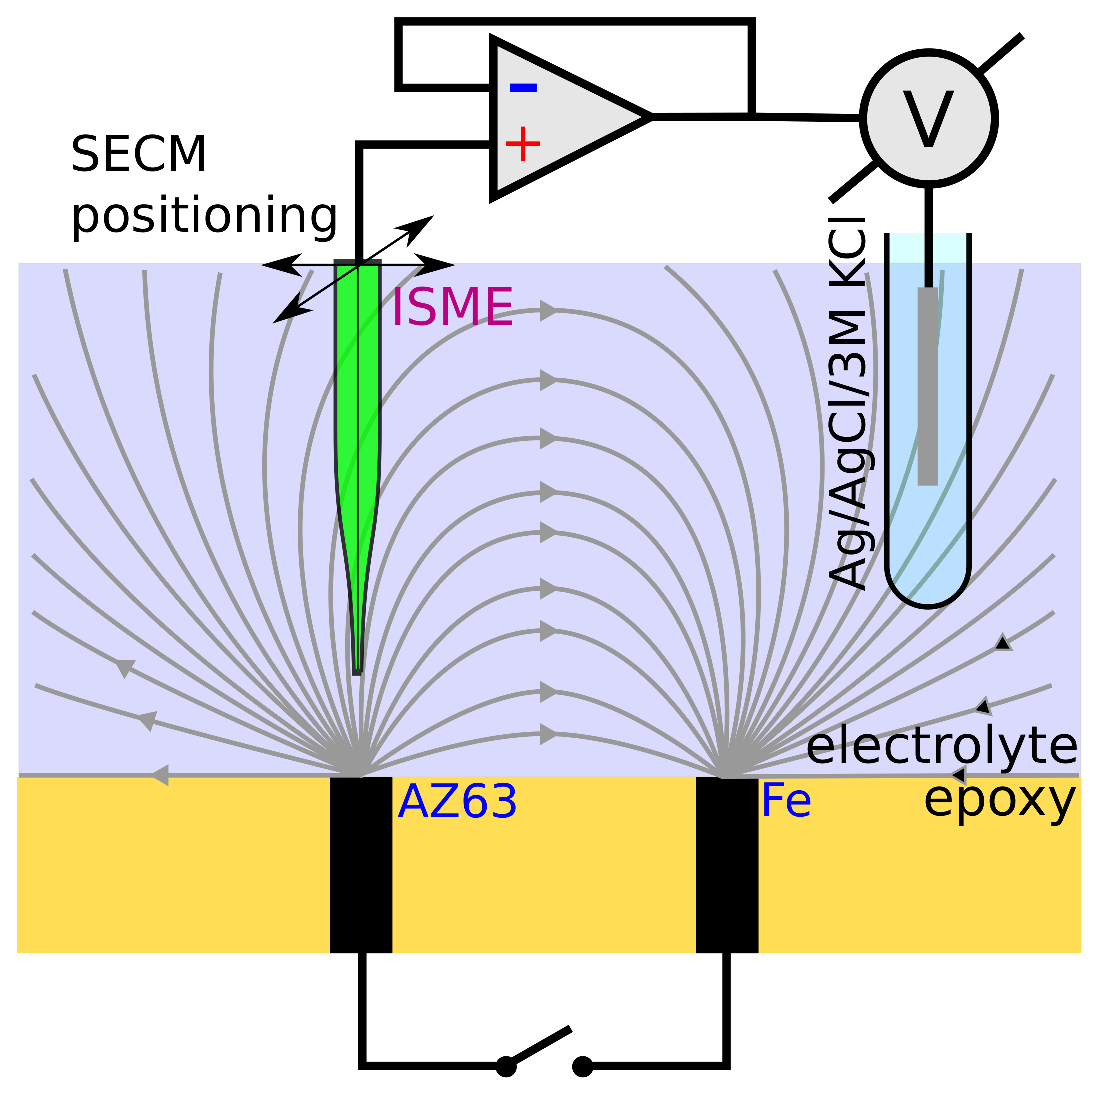
\includegraphics[width=0.5\textwidth]{abstract.eps}
\caption{Caption.}
\label{fig:abstract}
\end{figure}

\section{Material and methods}
\section{Results and discussion}

First, consecutive approaching curves were recorded above the corroding AZ63 sample, while the galvanic connection with the iron sample was...

The moment the galvanic connection was established, there was an immediate rise of about 140 mV in the measured potential of the microelectrode [fig], which cannot possibly be attributed to the increase of $Mg^{2+}$ activity that far from the source. Also, a 140 mV rise would mean an increase of about 3.5 orders of magnitude in $Mg^{2+}$ activity in less then a second. Even if one argues it's possible 100 $\upmu$m from the source, it cannot be the case 1000 $\upmu$m from it. The only plausable explanation is that sudden change is due to the electric field formed between the two metals. 


\begin{figure}
\centering
\begin{tikzpicture}
\begin{axis}[ymin=-75, ymax=200, xmin=0, xmax=680, xlabel={time, s}, ylabel={E vs. Ag/AgCl/3 M KCl, mV}, clip marker paths=true, width=10cm, height=6cm, legend style={draw=none}, legend cell align=left]
\addplot [domain=-30:100, color=red, mark=*] table {on_off_100.txt};
\addplot [domain=-30:100, color=blue, mark=*] table {on_off_1000.txt};

%\node[black, above left] at (axis cs:0,-290) {pH 4};
%\node[black, above right] at (axis cs:0,-290) {pH 6};
%\addplot +[mark=none] coordinates {(0, -300)-.- (0, -100)};
%\draw [dashed, black] (axis cs:0,-300) -- (axis cs:0,-100);
%\addlegendentry{raw recording}
%\addlegendentry{$E = - 280 + 97 e^{-t/3.76}$}
%\addlegendentry{$E = - 280 + 97 (e^{-t/9} + e^{-t/0.5577})/2$}
\end{axis}
\end{tikzpicture}
\caption[Transient response of the antimony microelectrode to analyte activity step.]{Transient response of the antimony microelectrode to analyte activity step.
The measuring and reference electrodes were dipped into buffer solutions with pH = 4 before the measurements started, and pH = 6 at t = 0 s, respectively.
Eq. \ref{eq:rc} was fitted (red line) on the measurement (gray marks) from the pH step to the end of the curve when potential reaches equilibrium in the pH = 6 buffer.}
\label{fig:transient}
\end{figure}





%%%%%%%%%%%%%%%%%%%%%%%%%%%%%%% FIGURE EXAMPLE %%%%%%%%%%%%%%%%%%%%%%%%%%%%%%%%%%
\def\s{0.25}
\begin{figure}
\centering
% trim = top left bottom right
\includegraphics[trim = 10mm 20mm 0mm 10mm, clip, width=\s\textwidth, angle=-90]{gnuplot_2d.eps}\includegraphics[trim = 10mm 20mm 0mm 10mm, clip, width=\s\textwidth, angle=-90]{gnuplot_2d.eps}\includegraphics[trim = 10mm 20mm 0mm 10mm, clip, width=\s\textwidth, angle=-90]{gnuplot_2d_deconvoluted.eps}
\caption{Caption.}
\label{fig:label1}
\end{figure}

%%%%%%%%%%%%%%%%%%%%%%%%%%%%%%% TABLE EXAMPLE %%%%%%%%%%%%%%%%%%%%%%%%%%%%%%%%%%
\begin{table}
                \caption{Comparison of the scanning algorithms.}
                \label{table:comp}
                \centering
                \begin{tabular}{r c c c}
                        Algorithm & Number of sampling points & Total scan time (s) & Mean squared error \\
                        \hline
                        Meander & 441 & 440 & $2.75\times 10^{-2}$ \\
                        Fast comb & 441 & 520  & $2.07\times 10^{-2}$ \\
                        Comb & 441 & 881 & $2.75\times 10^{-2}$ \\
                        Web & 110 & 109 & $9.63\times 10^{-3}$ \\
                        Arc & 341 & 340 & $2.95\times 10^{-3}$ \\

                \end{tabular}

\end{table}

\section{Conclusions}
\section*{Acknowledgements}
This research was supported by the European Union and the State of Hungary, co-financed by the European Social Fund in the framework of T\'{A}MOP-4.2.4.A/ 2-11/1-2012-0001 'National Excellence Program' and T\'{A}MOP-4.2.2.A-11/1/KONV-2012-0065.

\section*{References}

\begin{thebibliography}{5}

\bibitem{artefacts}P. J. Eaton, P. West. Atomic force microscopy. Vol. 10. Oxford: Oxford University Press, 2010.

\end{thebibliography}

\end{document}
